\documentclass{beamer}
%pacchetti
\usepackage[T1]{fontenc}
\usepackage[utf8]{inputenc}
\usepackage{graphicx}
\usepackage[italian]{babel}
\usepackage{mathrsfs}
\usepackage{booktabs}
\usepackage{amsmath}
\usepackage{amsfonts}
\usepackage{amssymb}
\usepackage{amsbsy}
\usepackage{amsthm}
\usepackage{enumerate}
\usepackage{quoting}
\quotingsetup{font=small}
\usepackage{diagbox}
\usepackage{graphicx}
\usepackage{setspace}
\usepackage{float}
\usepackage{version}
\usepackage{multicol}
\usepackage{beamerfoils}

\usepackage[none]{hyphenat} %avoid hyphenation
\usepackage{xcolor} %to uset \textcolor
% end pacchetti

\usetheme[bgphoto]{polimi}

% Full instructions available at:
% https://github.com/elauksap/beamerthemepolimi

% Set custom font (requires to compile with XeLaTeX).
\usepackage{ifxetex}
\ifxetex
\usepackage{fontspec}
\setsansfont[Scale=0.8]{Arial}
\fi

\usepackage{lipsum}


\newcommand\mynum[1]{%
	\usebeamercolor{enumerate item}%
	\tikzset{beameritem/.style={circle,inner sep=0,minimum size=2ex,text=enumerate item.bg,fill=enumerate item.fg,font=\footnotesize}}%
	\tikz[baseline=(n.base)]\node(n)[beameritem]{#1};%
}


\title{Is Dementia predictable?}

%\subtitle{Subtitle}
\author{F. Di Filippo, E. Manfrin, E. Musiari, E. Palli}
\date{17 december 2021}



\begin{document}

\begin{frame}
\maketitle
\end{frame}


\begin{frame}{Dataset}

Dataset Dementia and Alzheimer longitudinal
%\vspace{0.2 cm}
\begin{center}
	
	
	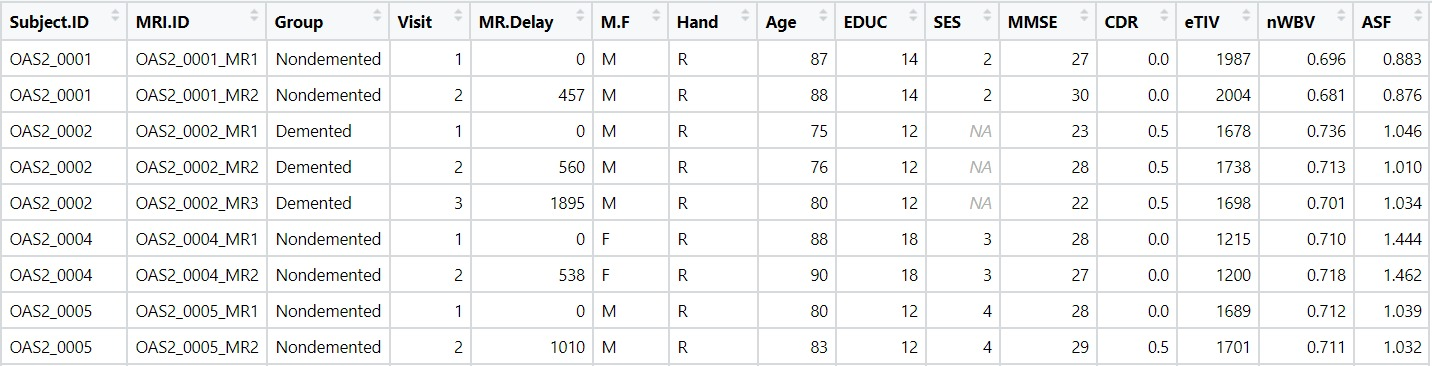
\includegraphics[width=\columnwidth]{dataset_al.jpeg}
\end{center}


where SES is Socioeconomic Status, MMSE is Mini Mental State Examination, CDR is Clinical Dementia Rating, eTIV is Estimated Total Intracranial Volume, nWBV is Normalize Whole Brain Volume and ASF is Atlas Scaling Factor.

\vspace{0.1 cm}
Source: Kaggle


\end{frame}

\begin{frame}{Analysis Male VS Female}
% tra demented e nondem
	
\end{frame}


\begin{frame}{Permutation}
% visita 1 vs 2

\end{frame}

\begin{frame}{Permutation}
% dem vs nondem

\end{frame}

\begin{frame}{2-ways manova}
% gruppi: m f dem nondem

\end{frame}

\begin{frame}{regression}

\end{frame}

\begin{frame}{regression}

\end{frame}

\begin{frame}{Prediction}

\end{frame}

\begin{frame}{Future questions}

\end{frame}


\end{document}